\let\negmedspace\undefined
\let\negthickspace\undefined
\documentclass[journal]{IEEEtran}
\usepackage[a5paper, margin=10mm, onecolumn]{geometry}
%\usepackage{lmodern} % Ensure lmodern is loaded for pdflatex
\usepackage{tfrupee} % Include tfrupee package

\setlength{\headheight}{1cm} % Set the height of the header box
\setlength{\headsep}{0mm}     % Set the distance between the header box and the top of the text

\usepackage{gvv-book}
\usepackage{gvv}
\usepackage{cite}
\usepackage{amsmath,amssymb,amsfonts,amsthm}
\usepackage{algorithmic}
\usepackage{graphicx}
\usepackage{textcomp}
\usepackage{xcolor}
\usepackage{txfonts}
\usepackage{listings}
\usepackage{enumitem}
\usepackage{mathtools}
\usepackage{gensymb}
\usepackage{comment}
\usepackage[breaklinks=true]{hyperref}
\usepackage{tkz-euclide} 
\usepackage{listings}
% \usepackage{gvv}                                        
\def\inputGnumericTable{}                                 
\usepackage[latin1]{inputenc}                                
\usepackage{color}                                            
\usepackage{array}                                            
\usepackage{longtable}                                       
\usepackage{calc}                                             
\usepackage{multirow}                                         
\usepackage{hhline}                                           
\usepackage{ifthen}    
\usepackage{lscape}
\begin{document}

\bibliographystyle{IEEEtran}
\vspace{3cm}

\title{NCERT 12.6.5.15}
\author{EE24BTECH11051 - Prajwal}
% \maketitle
% \newpage
% \bigskip
{\let\newpage\relax\maketitle}

\renewcommand{\thefigure}{\theenumi}
\renewcommand{\thetable}{\theenumi}
\setlength{\intextsep}{10pt} % Space between text and floats

\parindent 0px\textbf{Question}:Find two positive numbers $x$ and $y$ such that their sum is 35 and the product $x^2\times y^5$
is a maximum.

\solution\\
\textbf{Therotical logic:}
\begin{enumerate}
    \item Given
    \begin{align}
        x+y=35 , max(x^2\times y^5)=? \label{1}
    \end{align}
    \item Value of $x$ in terms of $y$ from  \eqref{1}
    \begin{align}
        x=35-y \label{2}
    \end{align}
    \item let $F(x,y)=x^2y^5$
    \item Substituting value of $x$ in equation $F(x,y)$ to convert it into single variable
    \begin{align}
        F(x,y)=x^2y^5 \label{3} \\
        F(y)=(35-y)^2y^5 \label{4} \\
        F(y)=(y^2-70y+1225)y^5 \label{5} \\
        F(y)=y^7-70y^6+1225y^5 \label{6}
    \end{align}
    Differentiate equation \eqref{6} with respect to $y$  set it to '0' for critical points
    \begin{align}
        \frac{dF}{dy}=7y^6-420y^5+6125y^4 \label{7} \\
        0=7y^4(y^2-60y+875) \label{8} \\
        0=7y^4(y-25)(y-35) \label{9}
    \end{align}
    \item From equation \eqref{9} critical points are $y=0,y=25\ \text{and}\  y=35$
    \item Differentiate equation \eqref{7} with respect to $y$ 
    \begin{align}
        \frac{d^2F}{dy^2}=7(6y^5-300y^4+3500y^3) \label{10}
    \end{align}
    \item If $\frac{d^2M}{dy^2}<0$ at a critical point,that is point of maximum 
    \begin{align}
        \frac{d^2F}{dy^2} \bigg|_{y=0} = 0 \label{11} \\
        \frac{d^2F}{dy^2} \bigg|_{y=25} =-27,343,750  \label{12} \\
        \frac{d^2F}{dy^2} \bigg|_{y=35} =105,043,750 \label{13}
    \end{align}
    \item From equation \eqref{12} $y=25$ is the point of maximum
    \item Value of $x$ and $y$ at which maximum value of the $x^2y^5$ is 
    \begin{align}
        y=25 \label{14} \\
        x=35-y=10 \label{15}
    \end{align}
\end{enumerate}
\textbf{Computational Logic:} 
Using the method of gradient accent
\begin{align}
    y_{n+1}=y_n+h*F^\prime(y_n) \label{16} \\
\end{align}
from equation \eqref{7},
\begin{align}
    y_{n+1}=y_n+h(7y_n^6-420y_n^5+6125y_n^4)
\end{align}
where,
\begin{align}
    h=10^{-10}
\end{align}
\begin{figure}[h]
    \centering
    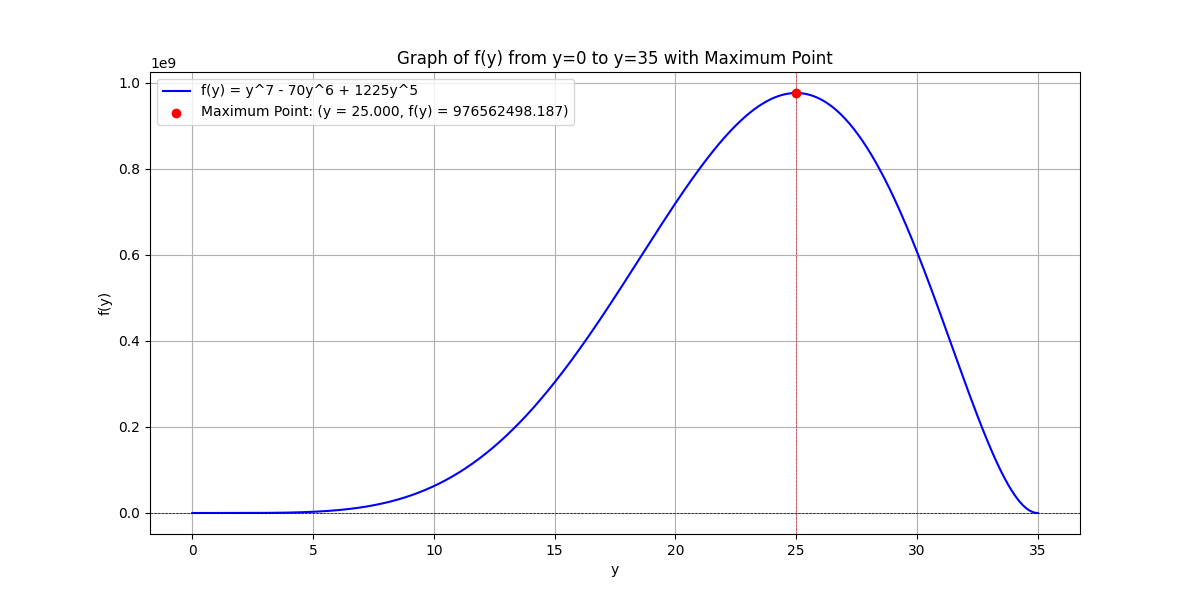
\includegraphics[width=\columnwidth]{figs/fig.png}
 \end{figure}


\end{document}
